\section{One-dimensional Chain}
\label{sec:1d-chain}

The analytical solution of the $T= 0$ \acs{1D} Hubbard model indicates that there is no Mott transition \cite{lieb_absence_1968} in the ground state, independently of the value of the on-site interaction $U$.
Consider the $\frac{U}{t} \gg 1$ limit. 
Then, the Hubbard model can be replaced by an effective atomic Heisenberg model defined in the Hilbert subspace with one electron per site, and antiferromagnetic order sets in.
At zero temperature, it is found that upon decreasing $U$, the system remains an antiferromagnetic insulator down to $U \rightarrow 0$, becoming a conductor only at $U = 0$.
Thus, we expect signs of antiferromagnetic for all $U$ for high enough $\beta$.
Upon decreasing $\beta$, thermal fluctuations tend to destroy long range order.
Conversely, as $\beta$ is increased, we expect to see a divergence in $\chi$, corresponding to a phase transition to the antiferromagnetic ground state.
We identify it by studying the spin-spin correlator $\left\langle S^z_i S^z_j \right\rangle$.
Fourier transforming, we obtain a peak at $q = \pi$ in the magnetic structure factor $S ( q ) $, and in the magnetic susceptibility $\chi (q)$.
For the case of the latter, the peak is found to increase in magnitude, and seems to diverge at $T = 0$.

\begin{figure}[H]\label{fig:divergences}
\hspace{0.3cm}
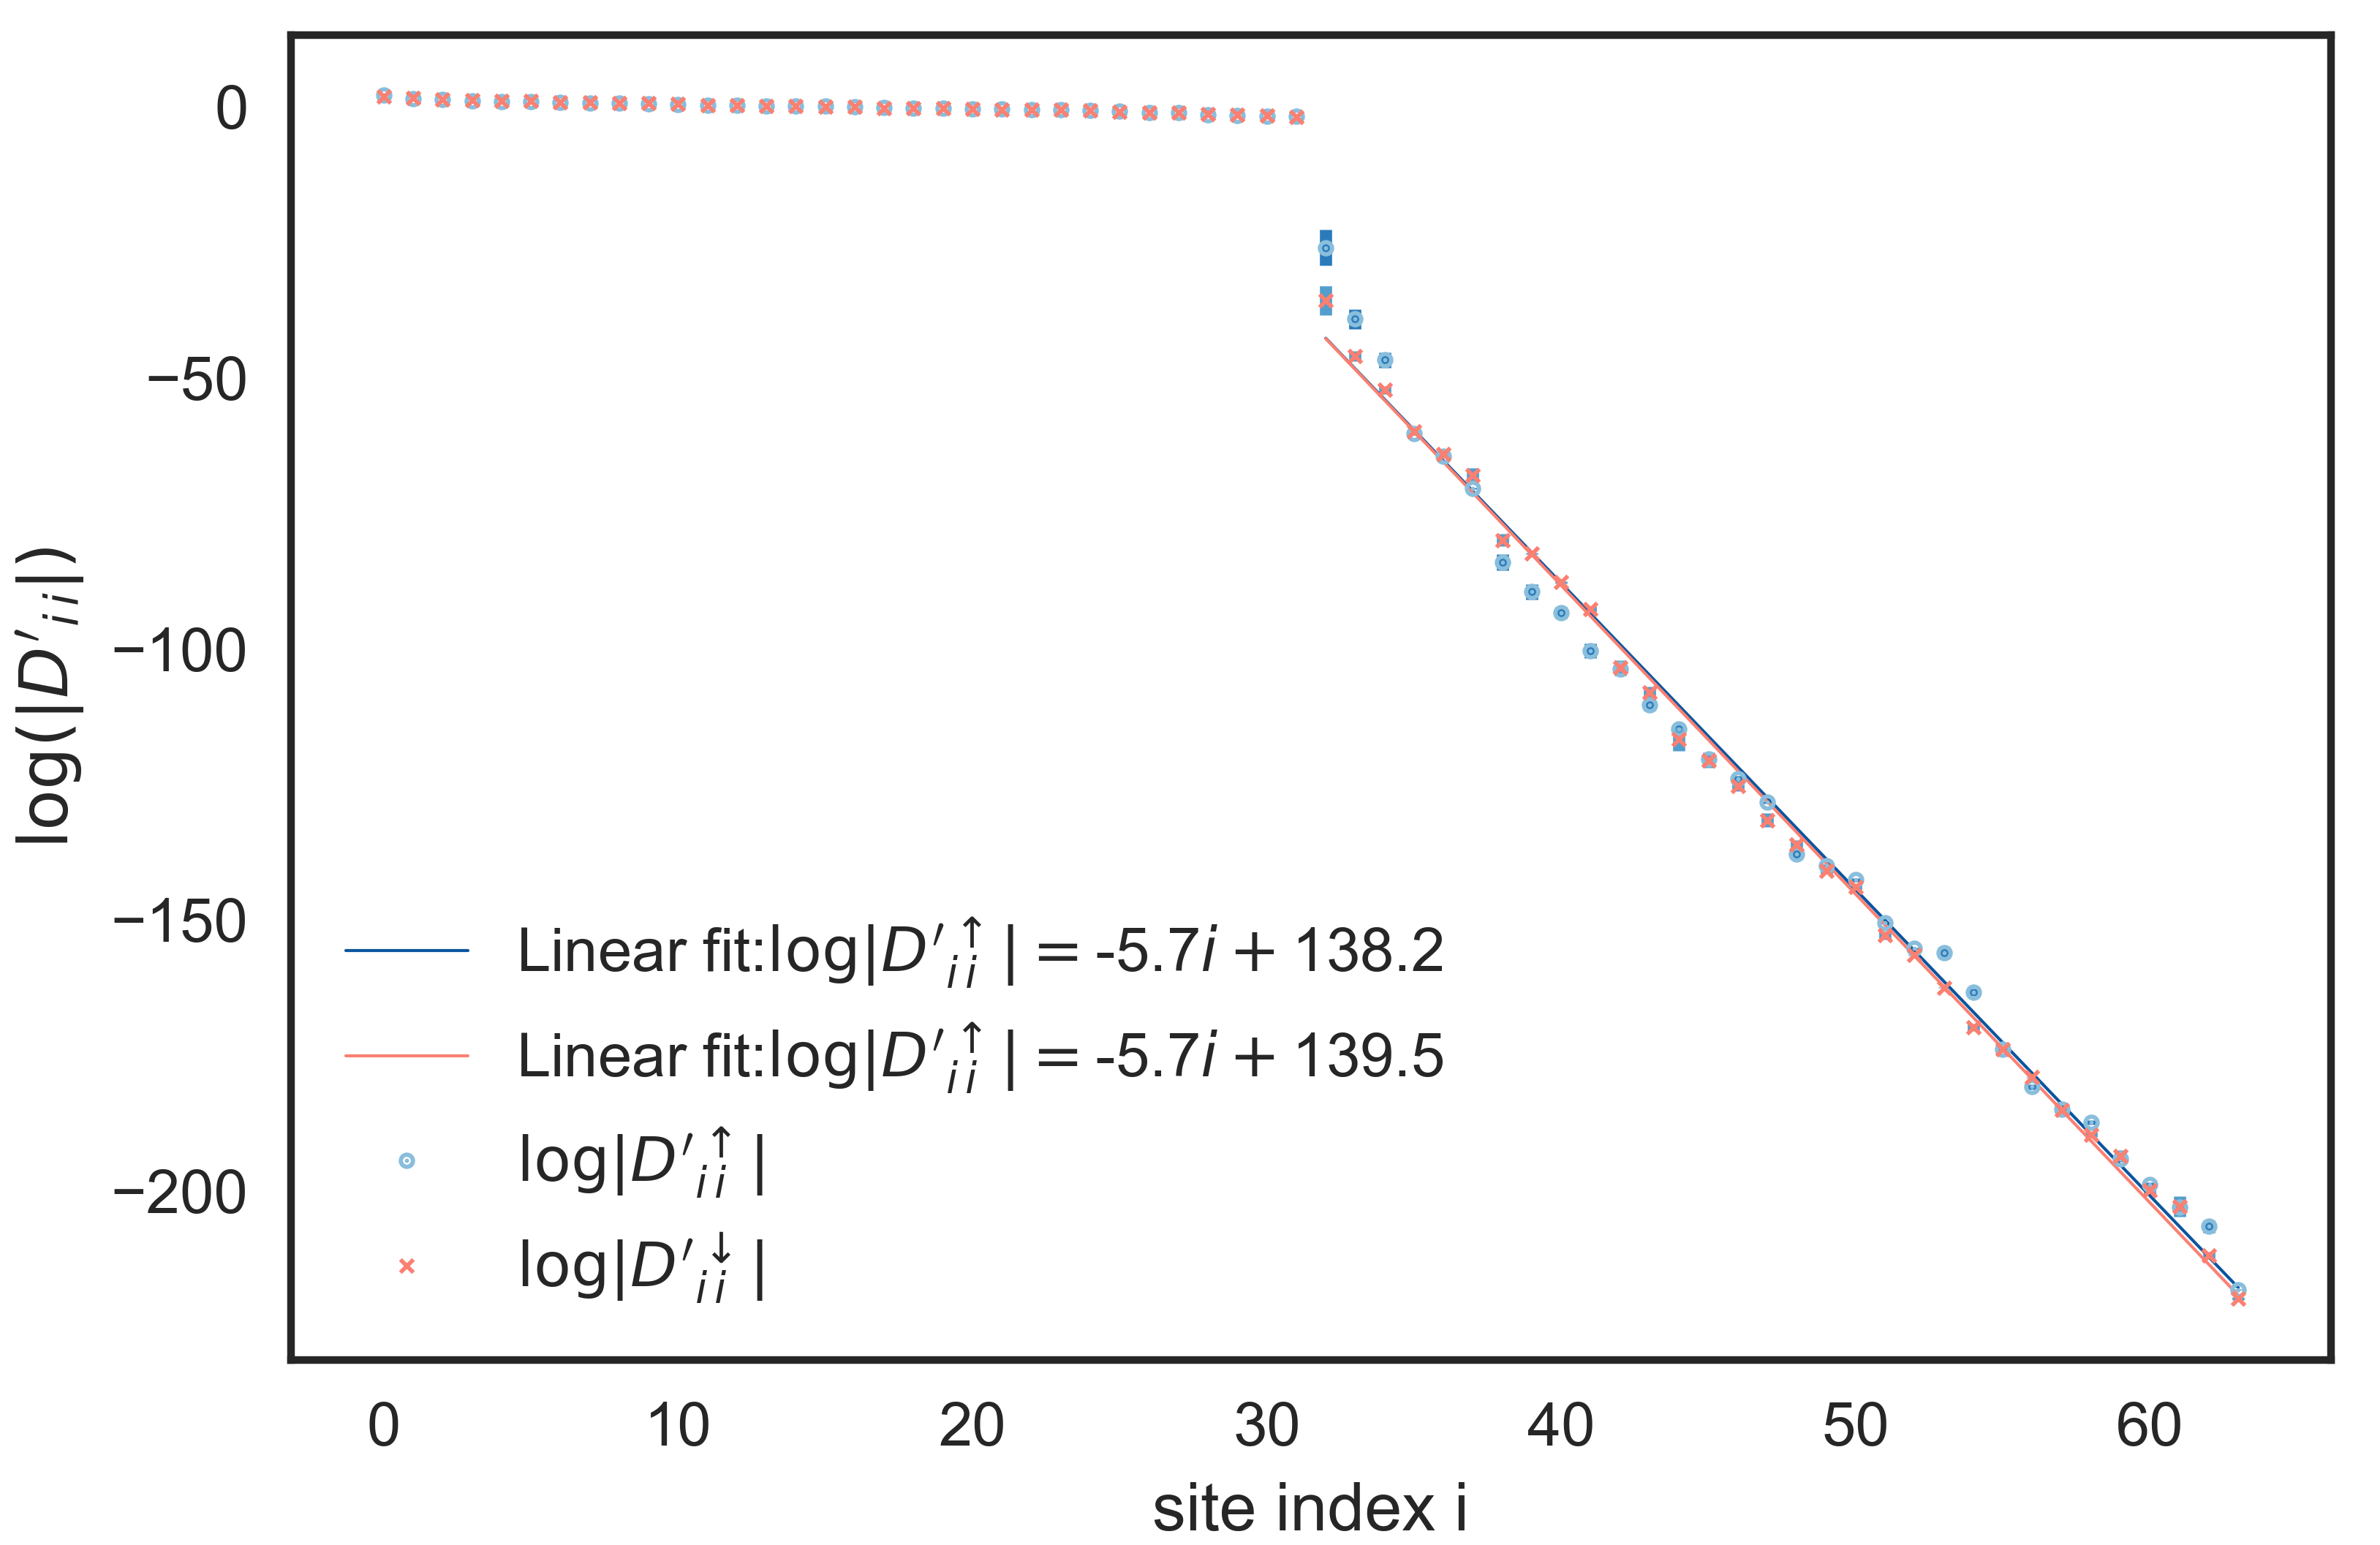
\includegraphics[scale=0.55]{Afqmc/OrdersOfMagnitude_N=64sites.png}
\hspace{0.3cm}
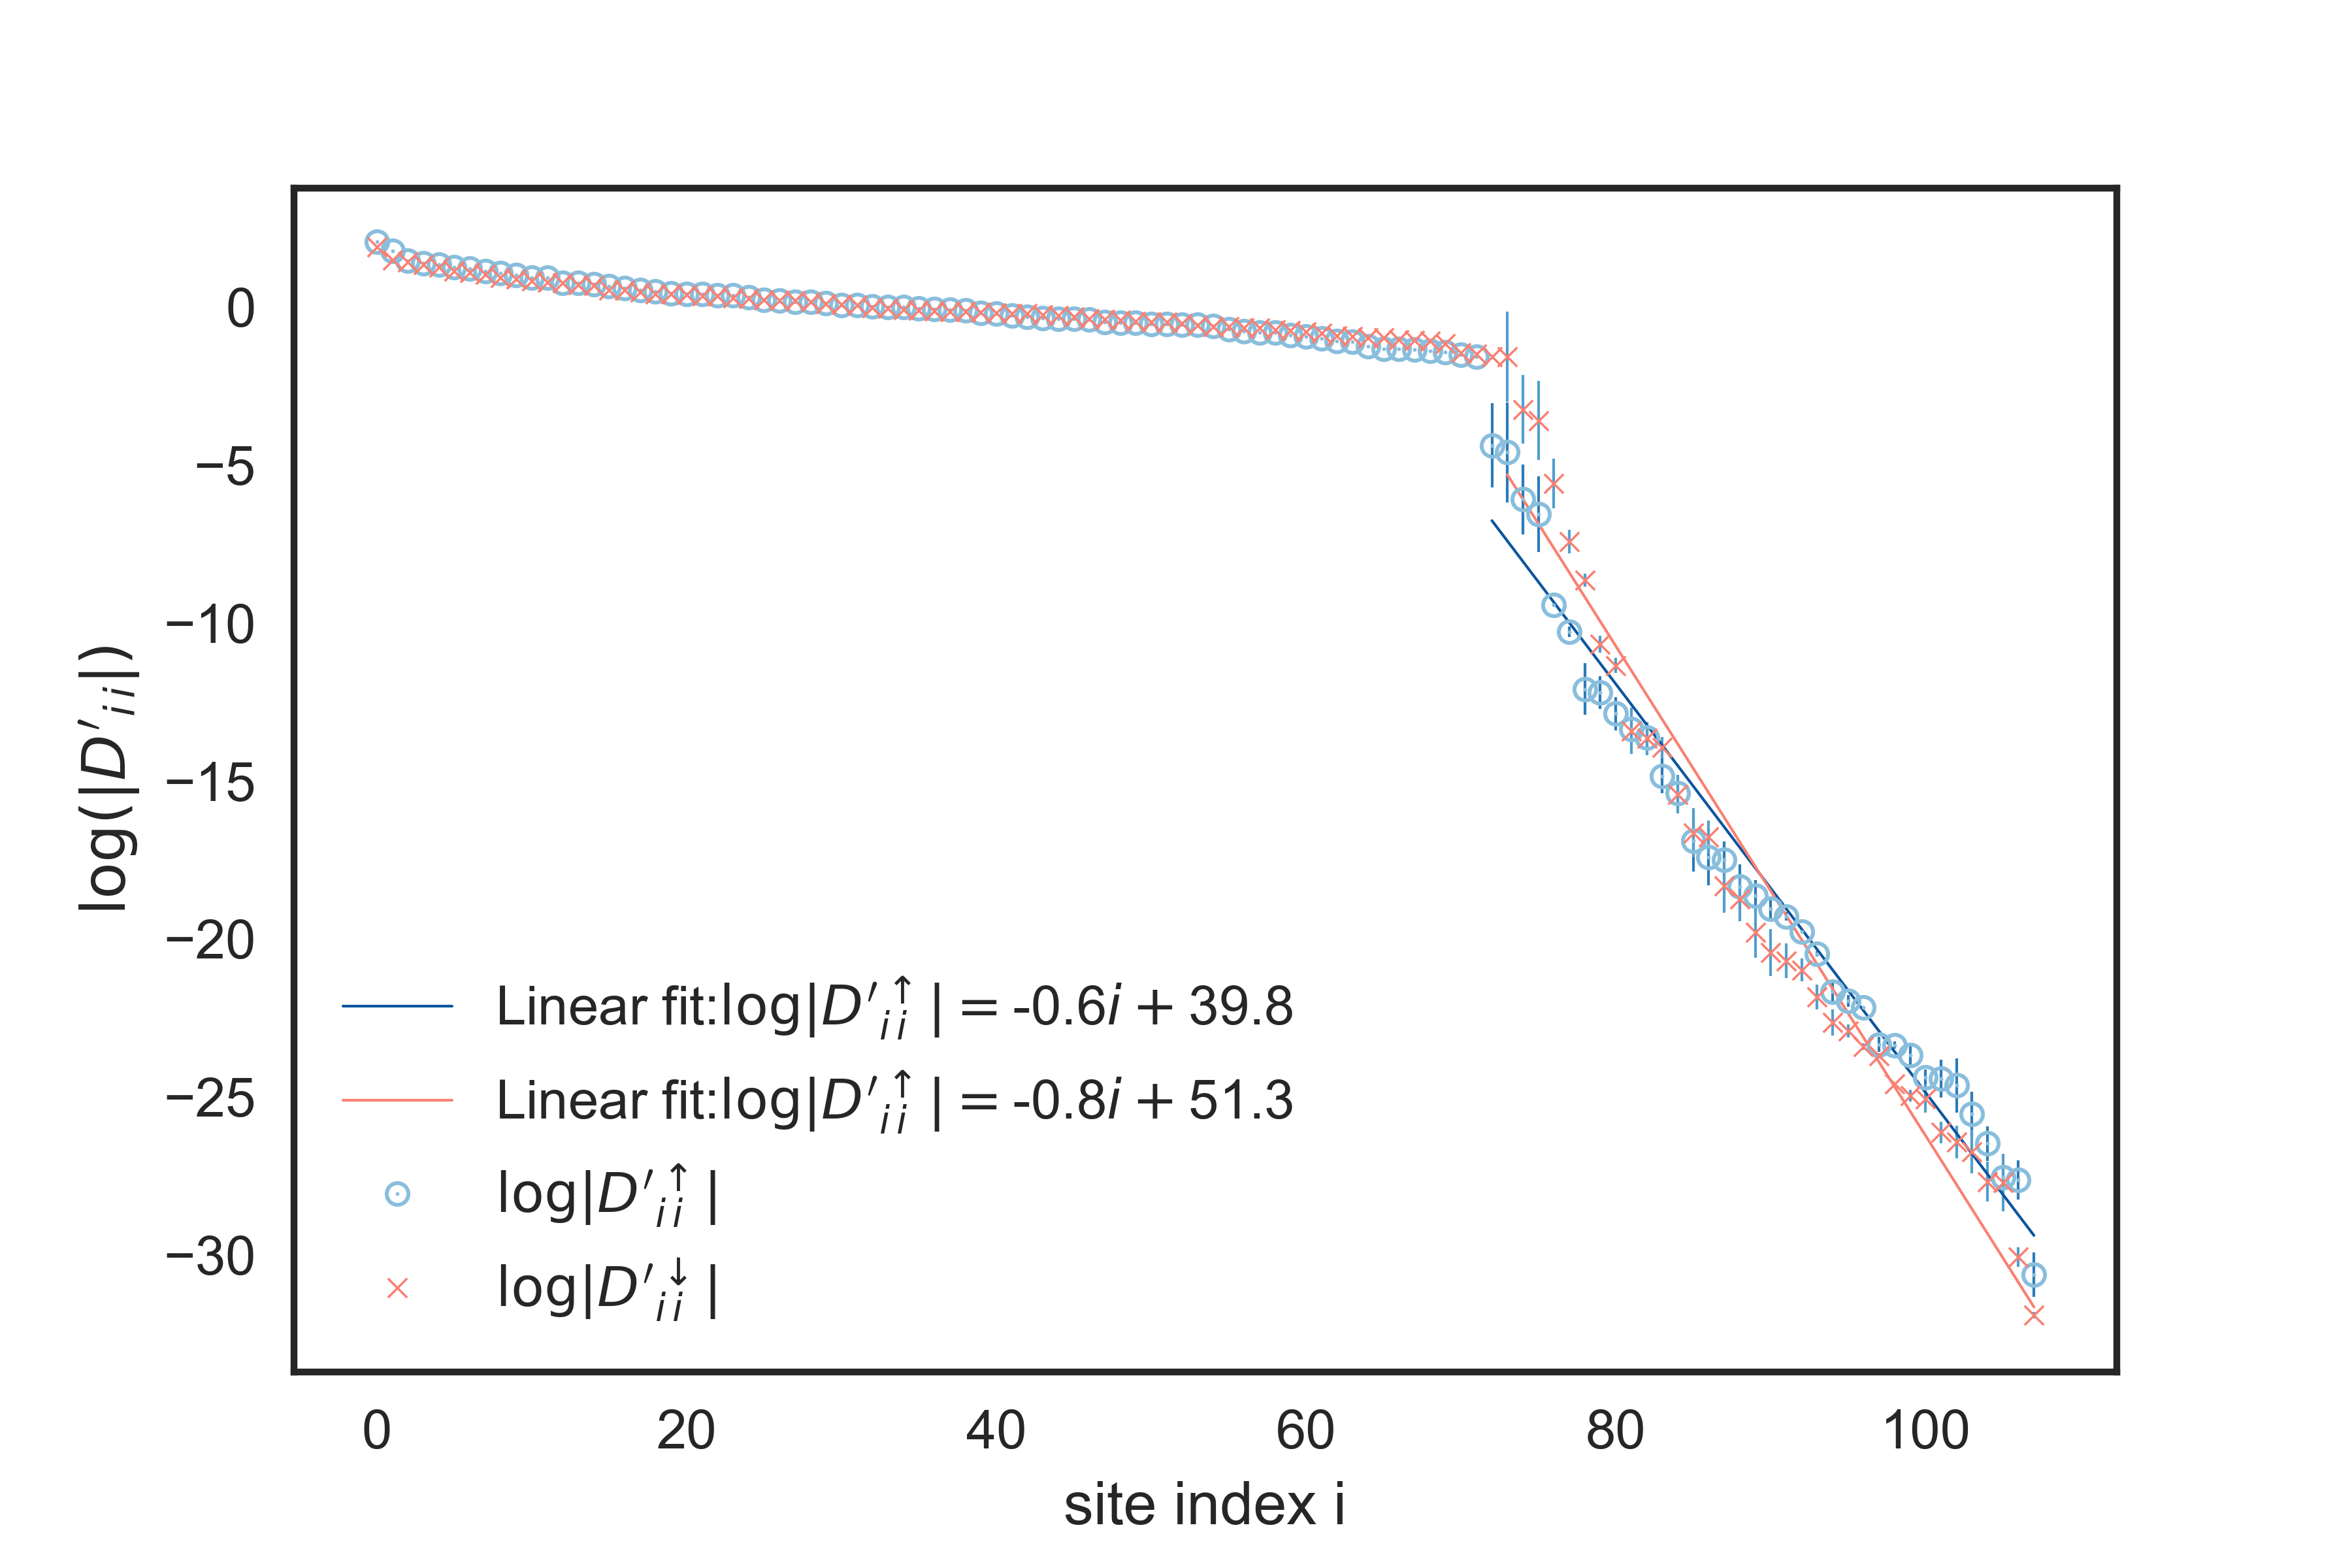
\includegraphics[scale=0.55]{Afqmc/OrdersOfMagnitude_N=108sites.png}
\caption[Exponentially divergent diagonal entries of $\bm D'$, showing the orders of magnitude spanned by the matrix elements of the stabilized matrix product.]{Exponentially divergent (and order one)  diagonal entries of $\bm D'$, showing the orders of magnitude spanned by the matrix elements of the stabilized matrix product.
The depicted systems are the same of Fig.(3.1). }
\end{figure}